
%%%%%%%%%%%%%%%%%%%%%%%%%%%%%%%%%%%%%%%%%%%%%%%%%%%%%%%%%%%%%%%%
\chapter{Introduction}
% \epigraph{\emph{``The computer is incredibly fast, accurate, and stupid. Man is unbelievably slow, inaccurate, and brilliant. The marriage of the two is a challenge and opportunity beyond imagination.''}}{-- Stuart G. Walesh, \citeyear{walesh1989urban}}
\bigskip

In this chapter, the reader is introduced to the topic of the thesis which includes general concepts, ideas, recent advances, and challenges.

%%%%%%%%%%%%%%%%%%%%%%%%%%%%%%%%%%%%%%%%%%%%%%%%%%%%%%%%%%%%%%%%
%%%%%%%%%%%%%%%%%%%%%%%%%%%%%%%%%%%%%%%%%%%%%%%%%%%%%%%%%%%%%%%%
\section{Background}\label{intro-background}

Biology is the interdisciplinary field of study coupling the knowledge and techniques of the mathematical, physical, and chemical sciences to describe the natural world and the life that inhabits it. Biological knowledge for most of the \nth{20} century was primarily discovered through reductionist techniques, which revealed the observed behavior and structure of cellular components. However, the rise of genomics in the 1990s has significantly changed the biological sciences by opening the door to more paths of inquiry via the increase in available data \citep{Palsson2000}. Of note are the \acrfull{HT} technologies being used to generate considerable amounts of data which are becoming more difficult to analyze and understand \citep{Sboner2011}. With increasing amounts of data available for researchers, there are emerging methods and techniques that can be leveraged to better understand the biological processes underpinning the behaviors and function of biological organisms and molecules.

In this section, the reader will be introduced to the fields of network theory,  systems biology,  and biostatistics and their respective ideas and concepts. With these concepts in mind, the reader should have the basic knowledge to understand the scopes and applications of the thesis. Section \ref{intro-network} covers the network and graph theory and its practical uses in systems research. Section \ref{intro-sysbio} describes the emergence of systems biology research and the resulting use of \textit{in silico} modeling.  Section \ref{intro-statml} discusses statistical and machine learning methods that are \textbf{**Unsure what to say here, will come back**}




%%%%%%%%%%%%%%%%%%%%%%%%%%%%%%%%%%%%%%%%%%%%%%%%%%%%%%%%%%%%%%%%
\subsection{Graphs and Networks} \label{intro-network}
 In general, we use the term \textit{graph} or \textit{network} to describe a collection of objects and the information about their relationships between each other. We can use this method and the abstract mathematical formalism arising from graph theory to describe many real-world phenomena; even those that tend to become more complex. The application of networks in network science spans countless real-world problems and fields of study, thus making it a prominent interdisciplinary field of study. 
 
 A simple example is a social network where there is a collection of individuals, and the information describing the individuals connection to other individuals in the network. 

\subsubsection{Graph Theory} \label{intro-net-graph}

In 1736, the famed mathematician Leonhard Euler published the first known paper on what would become the foundation of graph theory \citep{Euler1736}. His formalism tackled the problem known as the Seven Bridges of Königsberg. The city of Königsberg had three land masses with seven bridges connecting them as shown in Figure \ref{fig:konigsberg}. Euler proved that there was no path to go across all of the bridges only one time each. The modern interpretation of his abstract formalism defines the land masses as nodes (vertices, $\V$), and the bridges as links ($E$, or edges). His reason for there being no solution was based upon the number of points and the number of connections attached to each point. 

\begin{figure}[t]
    \centering
    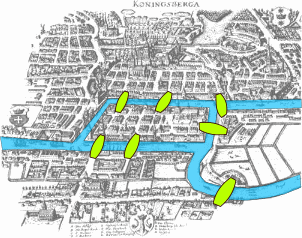
\includegraphics[scale = 0.75]{figure/background/Konigsberg_bridges.png}
    \caption[An image depicting the Seven Bridges of Königsberg problem. The land masses are defined as  nodes, and the bridges (in green) are defined as edges.]{An image depicting the Seven Bridges of Königsberg problem. The land masses are defined as  nodes, and the bridges (in green) are defined as edges. This image is licensed under the under the CC BY-SA 3.0 license \citep{Giusca2005}.}
    \label{fig:konigsberg}
\end{figure}

It is important to note that the terms \textit{network} and \textit{graph} in graph theory and network science are more-or-less synonymous. Technically, the mathematical description in graph theory describes a graph $\bm{G}(\V,E)$ that uses the form: \{\textit{graph}, \textit{vertex}, \textit{edge}\}. On the other hand, network science describes real-world systems which are of the form: \{\textit{network}, \textit{node}, \textit{link}\} \citep{Barabasi2016}. Thus, \textit{network} and \textit{graph} and their associated properties will be used interchangeably going forward. 

%Insert image of graph structure example?
As stated above, a graph $\bm{G}$ is defined as $\bm{G}(\V,E)$ and containing the nodes and respective set of edges. Initially, graphs may be split into two different types: \textit{undirected} and \ital{directed} graphs. These describe the directionality of the edge connecting vertex $i$ to vertex $j$ which has a given weight $w_{ij}$. In \ital{undirected} networks, the edge direction is not important, and the emphasis is placed on the relationship that vertex $i$ is connected to vertex $j$ with a given weight $w$. In \ital{directed} networks, the order from $i$ to $j$ is important, and is fundamental to the structure of the network. These networks can either be \ital{weighted} or \ital{unweighted}. The $w_{ij}$ values in \ital{weighted} networks vary based upon the weights associated with the connection, whereas the $w_{ij}$ values in a \ital{unweighted} network are set to 1. 

A graph may be depicted in one of three ways: 1) A \textbf{square adjacency matrix} $A$, which depicts all of the possible edges connecting vertex $i$ to vertex $j$ with a given weight $w_{ij}$ (so $A_{ij} = w_{ij}$). In this case, a directed network may be asymmetrical due to different edges connecting nodes with varying weights. An undirected network will always be symmetrical since the path from $i$ to $j$ does not matter which direction it goes in. 2) An \textbf{edge list} listing all of the nonzero edges in the network. This method usually describes the graph in a list where each entry takes the form: \{node $i$, node $j$, $w_{ij}$\}. It is commonly used in computational approaches because a majority of graphs are sparse and not fully connected, so edge lists reduce the computational  3) A \textbf{graphical representation} where nodes are points in the graph, and edges are depicted as lines between nodes. The graphical representation is up to the individual to change, but common implementations will change node sizes based on the number of edges connecting them, and modify edge width based upon the value of the weight.

\subsubsection{Network Science}
From the basic principles of graph theory being applied to real-world phenomena, network science emerged as a new field of study. As mentioned in Section \ref{intro-net-graph}, networks are graph-based systems that describe interacting agents in the world around us. As a field of study, network science is relatively new -- emerging in mainstream science only recently towards the end of the 1990s. 

Prior to this in the late 1950s,  Erd\"{o}s and  R\'{e}nyi introduced a paper on \ital{random graphs}, which describe networks whose nodes have probabilities $p$ of connecting to other nodes in a network \citep{Erdoes1959}. Networks at this point were regarded as regular with uninteresting topology and features, or very complex and random as associated with random graphs \citep{Vespignani2018}. It was not until 1998 when Watts and Strogatz proposed a new model called the \ital{small-world} network \citep{Watts1998} which defined a middle ground between a regular and random network. This model was better at describing the small average \ital{path length}\footnote{ Path length is defined as the shortest path between two nodes in a network. Average path length $l_G$ is defined as: $l_G=\frac{1}{n (n-1)}\sum_{i\neq j} d(v_i,v_j)$ where $d(v_i,v_j)$ is the distance between vertices $v_i$ and $v_j$.} 
of real-world networks and nodes that were more connected than others. Interestingly enough, the next paper to fully push network science into many domains was when Barab\'{a}si and Albert published their papers in 1999 on preferential-attachment and power laws \citep{Barabasi1999_emergence,Barabasi1999_mean_field,Albert1999}. The degree distributions of many systems follow power-law distributions, and are `heavy-tailed' compared to the normal distribution of random graphs. 

From here, specialists across all types of disciplines started to implement network science based analyses of their field of study. For example, some of these fields range between sociology (social network analyses), biological systems (epidemiological models, \acrfull{GRNs}, etc.), information-technology networks (\acrfull{WWW}), and countless other disciplines. Barab\'{a}si expresses the interdisciplinary nature of network science quite well:

\begin{displayquote}
``Today many fields consider network science their own. Mathematicians rightly claim ownership and priority through graph theory; the exploration of social networks by sociologists goes back decades; physics lent the universality concept and infused many analytical tools that are now unavoidable in the study of networks; biology invested hundreds of millions of dollars into mapping subcellular networks; computer science offered an algorithmic perspective, allowing us to explore very large networks; engineering invested considerable efforts into the exploration of infrastructural networks. It is remarkable how these many disparate pieces managed to fit together, giving birth to a new discipline.''

\rightline{{ \rm -- \citet{Barabasi2016}}}
\end{displayquote}
Appreciating the scope of network science research presented in the previous quote is helpful when approaching a novel problem, because a technique developed in one of the many applicable fields may be a suitable technique for the current problem. 

\subsubsection{Complex Systems}\label{intro-complex-sys}
In the last couple of decades, the growth of network science also led to the growth and study of complex systems. \ital{Complex system} is a name generally given to agents, organisms, structures, and other phenomena that exhibit emergent behaviors and properties \citep{Foote2007}. \textbf{following sentence is required. should it be rewritten, or what is the proper grammar/punctuation structure:} Such objects and systems tend to be, as the name suggests, complicated as they often are not fully deterministic due to chaotic and non-linear interactions. A term most often associated with complex systems is \textit{emergence}, which describes the unexpected outcomes from the system. 

Emergence arises because the properties of an individual agent in a system may be fully known, but as we examine the interactions between multiple interacting agents in a network, it is often not possible to study and predict the exact outcomes from each interaction. Such behaviors are found frequently in real-life, and the role of complexity science has been to take these instances and try to understand them with old and new theoretical techniques. One of the most important characteristics of these systems is the fact that the interactions between agents can be anything from an exchange of energy, to momentum, material or information \citep{Werner1999}, which allows for most experimental and some theoretical problems to be explored and further researched. Note that emergent behaviors in complex systems are often \textit{robust} -- meaning that even if some microscopic interactions are rewritten, the ultimate behavior of the system is similar. Robustness is a fundamental property of complex systems because if these systems were not robust their behaviors would be much more predictable and the causal mechanisms driving the behavior would be more apparent. In this case we would probably no longer need to use complexity theory techniques to understand these phenomena. 

Complex systems are often described by network science and graph theory methods since they are able to be described by networks, but the tools that are used to investigate them vary quite largely. Some common tools used to describe and research the systems take a bottom-up approach or a top-down approach \citep{Mhamdi2018}. A typical type of bottom-up approach would be agent-based modeling, where individual agents are defined and given certain probabilistic characteristics and behaviors. Then their interactions within the model can be modeled based upon the unique agent's behavior, while interesting metrics are recorded as the simulation runs. Another bottom-up approach would be the use of cellular automata as they are similar to agent-based models where the immediate surroundings of an individual impact its behavior. Together these microscopic interactions turn into some type of macroscopic behavior that we would define as an emergent behavior. Top-down approaches look at known causal mechanisms and behaviors of individual interactions that can be represented via numerical and analytical nonlinear dynamical systems. In the case of an analytical description of the system, we would expect the result to differ drastically from the complex system's actual behavior since it would generalize the inherently large parameter space. Using numerical methods would allow for the parameters of the system to be better identified because the dynamics might not have analytical solutions or be described with a close-form solution. The top-down approach is a more holistic approach since we try to generalize the behavior of the system through guiding equations.



%%%%%%%%%%%%%%%%%%%%%%%%%%%%%%%%%%%%%%%%%%%%%%%%%%%%%%%%%%%%%%%%
\subsection{Systems Biology} \label{intro-sysbio}
As mentioned previously, biology research has focused upon gaining new knowledge through reductionist techniques, but novel research into \acrshort{HT} technologies has increased the scope of biological research. Today, we find that biological research has extended to a more integrative approach that includes the use of integrative analysis, bioinformatics, mathematical models, and \textit{in silico} (computer simulation) models \citep{Palsson2006}. Together this is termed as systems biology, which extends beyond the component-based biology that reductionist techniques are derived from. 

\subsubsection{Network Structure and Emergent Functionalities} \label{ref:intro-emergent-function}
Since we have growing lists of information on cellular components derived from \acrshort{HT} technologies and we know that cells, biological molecules and structures lead to overall behaviors, with inductive reasoning we assume that there must be behaviors at the microscopic level that lead to macroscopic behaviors. Thus, we want to figure out how emergent cell behavior and functionality arise. A systems perspective allows us to first use the information and properties of our cellular components to then model interactions that lead to emergent behaviors and reveal functional roles of specific groups of cellular components. Figure \ref{fig-intro-systems} sketches out the difference between the \nth{20} and \nth{21}-Century approach to biology, and shows that the integrative approach of systems biology uses different methods that utilize the information provided by components biology. 
% A term used to describe this initial organization and investigation into cell function is \textit{cell circuit}.
\begin{figure}[ht!]
    \centering
    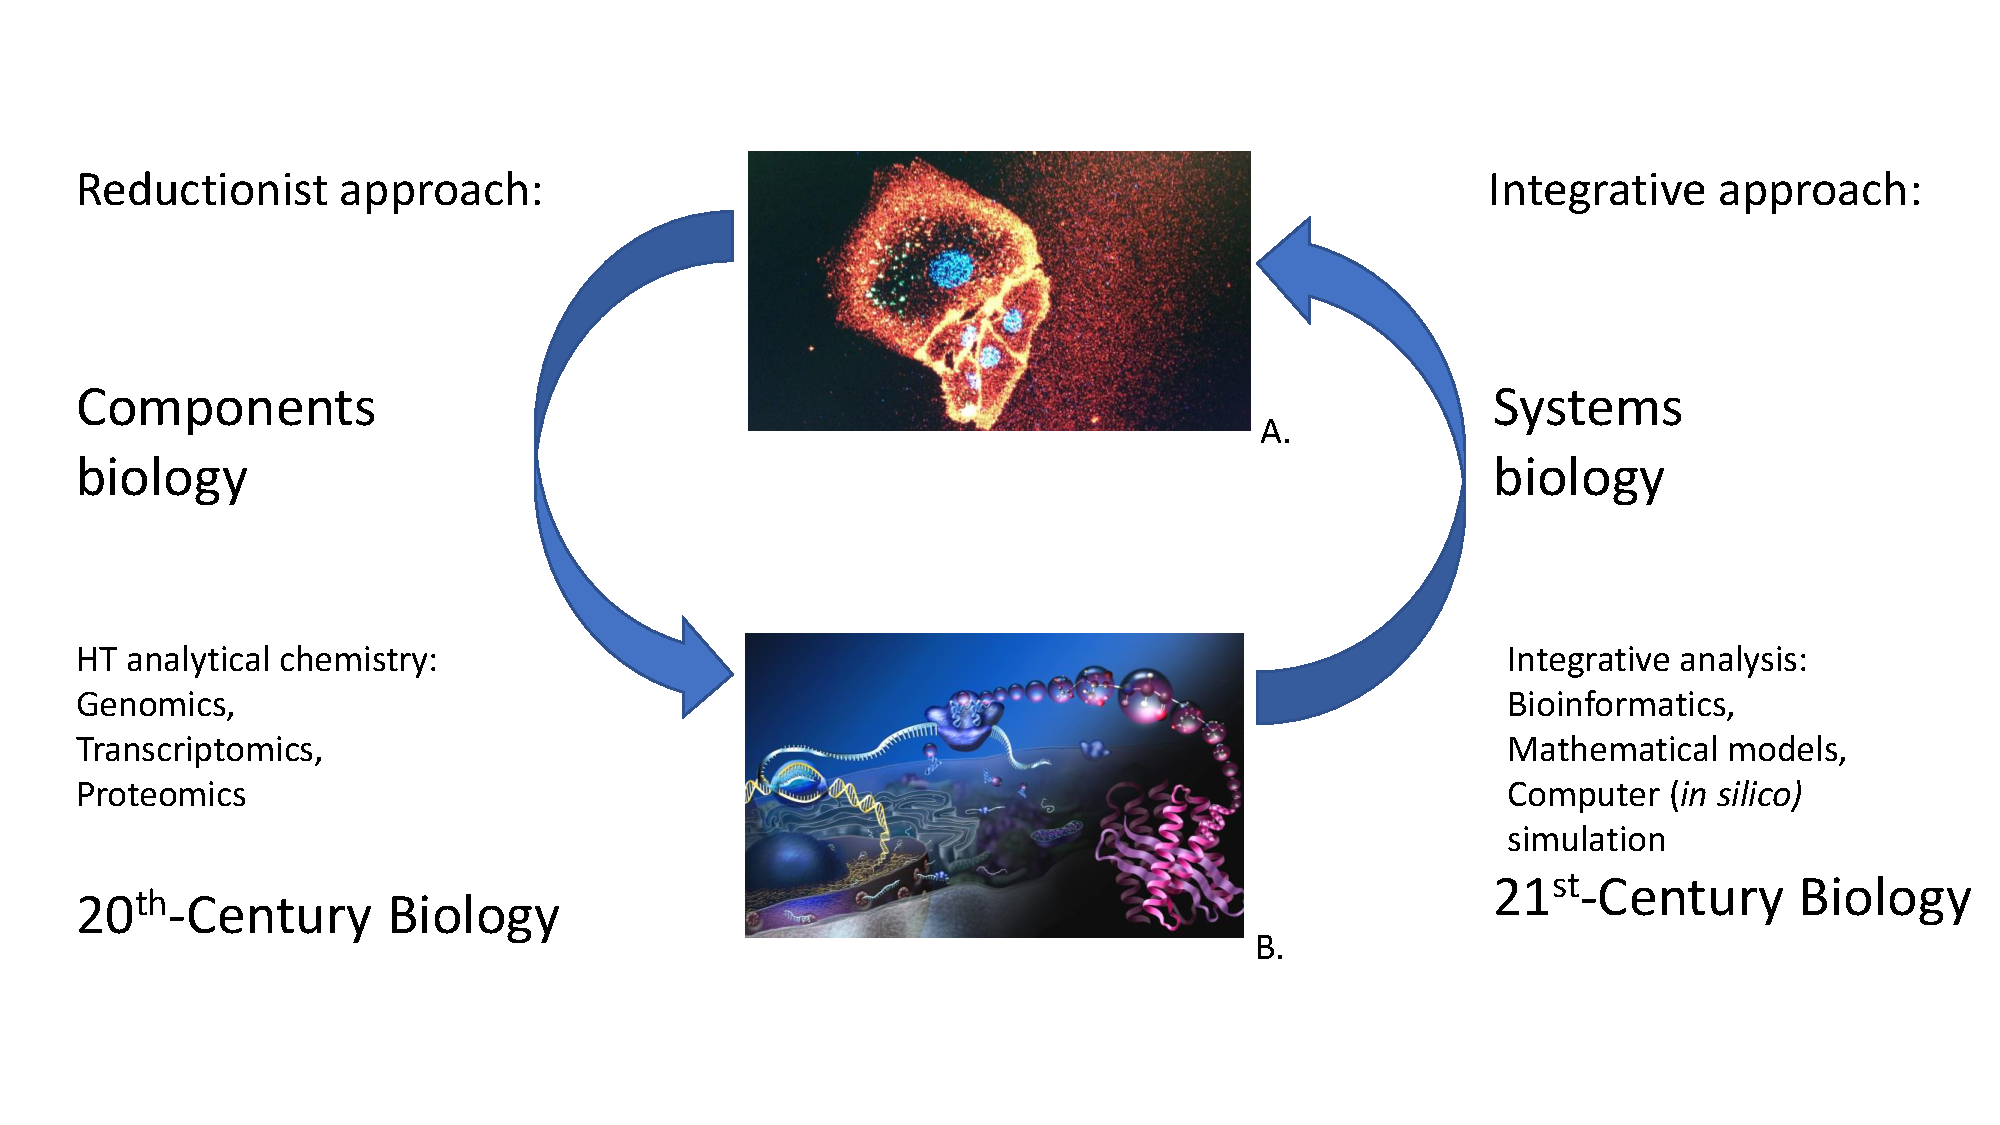
\includegraphics[width=1.0\linewidth]{figure/background/systems.pdf}
    \caption[Diagram indicating the \nth{20}-Century approach of reductionist biology, where biology is broken down into components. In this case we depict human cells (\textbf{A}), and an artist's depiction of different omics functions (\textbf{B}). With \acrshort{HT} technologies (such as the omics methods listed) emerging in the \nth{20}-Century, we have acquired the information necessary to know what makes up biological organisms. This has led to the integrative approach of systems biology and the work that is presently being performed today in the \nth{21}-Century.]{Diagram indicating the \nth{20}-Century approach of reductionist biology, where biology is broken down into components. In this case we depict human cells \textbf{A}, and an artist's depiction of different omics functions \textbf{B}. With \acrshort{HT} technologies (such as the omics methods listed) emerging in the \nth{20}-Century, we have acquired the information necessary to know what makes up biological organisms. This has led to the integrative approach of systems biology and the work that is presently being performed today in the \nth{21}-Century. The diagram was redrawn from \citet{Palsson2000,Palsson2006} and the subfigures \textbf{A} and \textbf{B} are available from \citet{Vidal2013} and \citet{Rager2012} respectively under Creative Commons licenses listed in their citations.}
    \label{fig-intro-systems}
\end{figure}

Overall, a system-level understanding of biological systems is dependent upon four properties: system structures, system dynamics, control methods, and design methods \citep{Kitano2002}. System structures are found via our components biology methods and represent gene interactions, biochemical pathways, and physical properties of biological structures. Insight into system structures today have been heavily dependent on laboratory experimentation, expression profiling, and transcription regulation analyses of \acrfull{mRNA}. System dynamics knowledge requires the construction of models based upon information related to system structure. In turn, model building requires the scope of the model to be defined prior. These are extremely complicated systems containing many parts, so the scope of the model requires a focus and a resolution level. Most models take similar forms to the approaches described in Section \ref{intro-complex-sys}. Control and design methods are rooted in discovering and designing mechanisms to control and modulate cell and biological system states in order to learn about the system as a whole \citep{Kitano2002}. Together these factors allow for different levels of a biological system's hierarchy to be linked. 

\textbf{This paragraph might need to come before the previous one.} Cellular functions related to the combined behavior of a group of system structures (genes in this case) make up the components that lead to system-level understanding. These functions are often defined as \textit{genetic circuits}, \textit{cellular wiring diagrams}, and modules \citep{Palsson2006}. We can build frameworks for modeling specific intracellular behaviors through genetic circuits, and then we can describe physiological behaviors as emergent functions of multiple genetic circuits. This type of process allows the systems approach to work because we can map function between the different circuit components. Utilizing this component-based approach means that the information produced by \acrshort{HT} technologies allow for the genome to actually be the system we are investigating and modeling. 

%%%%%%%%%%%%%%%%%%%%%%%%%%%%%%%%%%%%%%%%%%%%%%%%%%%%%%%%%%%%%%%%
%%%%%%%%%%%%%%%%%%%%%%%%%%%%%%%%%%%%%%%%%%%%%%%%%%%%%%%%%%%%%%%%
\subsubsection{Computational Biology as it Relates to Systems Biology} \label{intro-compbio}
Computational methods for modeling biological behavior have been around for nearly 60 years. Some of the first biological simulations were run on analog computers by \citet{Goodwin1963}.  \citeauthor{Goodwin1963} modeled the oscillatory behavior in \acrshort{GRNs} by exploring self-negative feedback loops for a gene that codes for the production of a metabolite that in turn inhibits the expression of the gene itself. This initial modeling led to many other studies using computers between the 1970s and the 1990s to simulate large metabolic networks, cell-scale models, genome-scale models of viruses, genome-scale metabolic models of bacteria, and large-scale models of mitosis \citep{Palsson2006}. The past twenty years have seen a significant increase in the scope of computational biology work, and most of this is due to the shift in computational capabilities as well as the ability to record more information from experiments and explore biology significantly better at the genome level. An interesting opinion from 2002 stated that biology is set to become a quantitative heavy science because the need for numerical analysis and modeling to discover system-wide analytical theories is necessary. They argue that qualitative thinking fails with the complexity of biological systems and are under the opinion that biology would become one of the most computer-intensive sciences this century \citep{Noble2002}. Observing the field today, it would be fair to say that they have been right so far about the role of computation in biology. Most academic and industrial biology research requires the aid of individuals well-versed in computational methods, for they help make sense of data from all hierarchy levels of the systems being investigated, and they play a large role in guiding research questions that are based on analyses and computational models.   

\textbf{this will probably go at the end for future methods}
In this thesis, systems and computational biology play a role in understanding the behavior of the gut microbiota. Current knowledge of the human gut microbiome is still in its infancy. There still exists a large need for metabolic pathways and flux balance analysis models to be created because the gut is comprised of so many microbes. Following the metabolites as they are fermented and generated remains a key piece to understanding microbiome influence on human health because ultimately it is the metabolites that are interacting with the human host. 

% \subsubsection{Prospects for Precision Medicine}
\subsection{Microbiology}\label{intro-micro}
As some of the most abundant and diverse life forms on the planet and despite being around for billions of years, human research of microorganisms only started in 1676 when Dutch scientist Antonie van Leeuwenhoek successfully created the first single-lensed microscopes and wrote on the presence of protists and bacteria living in different environments \citep{Lane2015}. His research created the field of microbiology which focuses on the study of biological entities that are too small to be seen by the unaided eye. These entities may include individuals from the Archaea, Bacteria, and Eukarya domains, and more specifically include bacteria, archaea, protists, fungi, parasites, and viruses \citep{Sattley2015}. While there are many different fields of study in microbiology, this thesis focuses on the ecological communities that microorganisms live in.

\subsubsection{Microbiota and the Microbiome}\label{intro-microbs}
Microorganisms can be found all over the earth inhabiting mundane and extreme places alike: from the upper parts of the atmosphere \citep{Fulton1966}
% soil, the bodies of other organisms, 
to high temperature and pressure environments of submarine hydrothermal vents \citep{Anderson2011}. In all of these environments microbial communities emerge and flourish as they compete and support each others metabolic systems. With new \acrshort{HT} technologies, the ability to study individual microbes and microbial systems has improved, and the application of systems biology techniques promises novel discoveries in the years to come.

To the casual observer the terms \textit{micobiota} and \textit{microbiome} appear to be interchangeable, but they have subtle differences. The term \textit{microbiota} is commonly used to describe the group of microorganisms in an environment \citep{Marchesi2015}. With this term we can discuss communities of microorganisms as microbiotic systems: e.g.\ the human gut microbiota, soil microbiota,  plant microbiota, etc. We use \textit{microbiome} to describe the entire habitat including the microorganisms, their genomes, and environmental conditions \citep{Marchesi2015}. Among the factors that can describe the microbiome are the multiple types of -\textit{omics} data including: \textit{metabolomics}, \textit{metabonomics}, \textit{metatranscriptomics}, and \textit{metaproteomics}.


\subsubsection{Microbial Definitions}\label{intro-mic-def}

We define a community of microbes as the \textit{microbiota}.


%%%%%%%%%%%%%%%%%%%%%%%%%%%%%%%%%%%%%%%%%%%%%%%%%%%%%%%%%%%%%%%%
\subsection{Statistical Learning and Machine Learning} \label{intro-statml}


\section{Analyzing Correlation Networks to Identify Differences in Comparable Networks}\label{intro-overall}

Connection of microbiome to complex systems: feedback systems, nonlinearity, hierarchical organization 

The aim of this thesis is to utilize more suitable statistical methods to generate correlation networks derived from compositional data. This work is focused specifically on the human gut microbiota, with a focus on comparing control (healthy) and case (diseased) cohorts. Since current knowledge of the human gut microbiota is derived from compositional data, we require formal methods to deal with compositional data that may contain both highly dominant and rare taxa. And since this compositional data may vary greatly between reads in the same sample or across labs, normalization methods must be utilized to allow for a comparison to be formulated.

Since the field is relatively new, the role of these types of microbial occurrences is unknown and thus  

